\chapter{DTLS} \label{Chp: DTLS}

In this chapter we analyse DTLS on Contiki. We consider only two ciphersuites those have been implemented by the tinydtls implementation, which are TLS\_PSK\_WITH\_AES\_128\_CCM\_8 and TLS\_ECDHE\_ECDSA\_WITH\_AES\_128\_CCM\_8. 

One thing to be noticed is that both ciphersuites uses AES-128 CCM for data encryption and therefore they only behave different during handshake. Hence we do not distinguish application data encrypted by both ciphersuites.

\section{Protocol and Implementation}

Due to the fact that tinydlts implemented only a minimum features of DTLS and supports only two ciphersuites, TLS\_PSK\_WITH\_AES\_128\_CCM\_8 and TLS\_ECDHE\_ECDSA\_WITH\_AES\_128\_CCM\_8, we have found no applicable attacks from \cite{rfc7457}.

\section{DTLS Handshake}

\textbf{[To be done...]}

\section{Packet Size}

Since application data are encrypted using AES-128 CCM, its size is not hidden and is visible in the header, as highlighted in the middle of \Cref{Fig: Size of application data in DTLS}.

\begin{figure*}[ht!]
	\center
	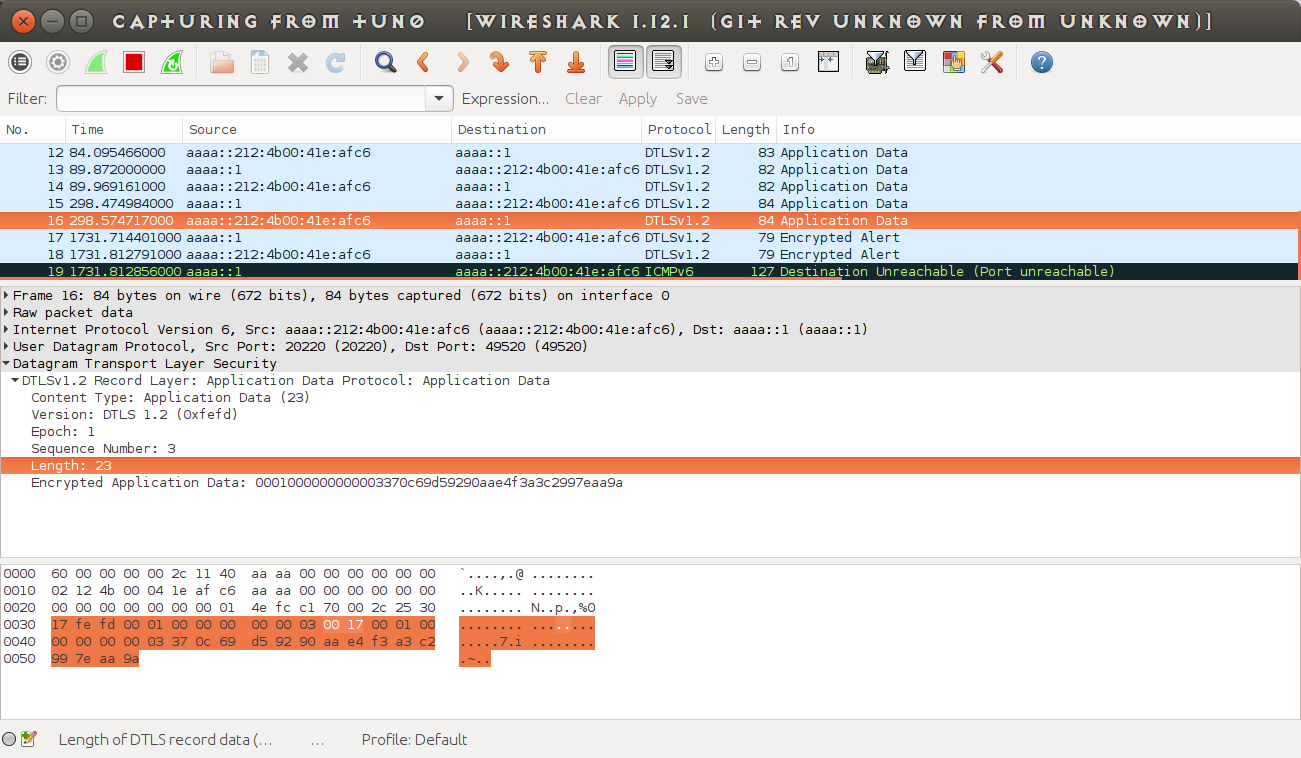
\includegraphics[width=.7\textwidth]{fig/dtlslength.png}
	\caption{Size of application data in DTLS}
	\label{Fig: Size of application data in DTLS}
\end{figure*}

Referring to \cite{rfc5116}, the size of application data is exactly the value of the highlighted Length in \Cref{Fig: Size of application data in DTLS} minus $16$ bytes.

%CoAP

\section{Timing}

In this section, we analyse the availability of timing information when the application data is protected by DTLS using the tinydtls implementation on Contiki.

\subsection{Processing Model}

The procedure of a Session with DTLS is as depicted by \Cref{Fig: A Session with DTLS}.

\begin{figure*}[ht!]
	\center
	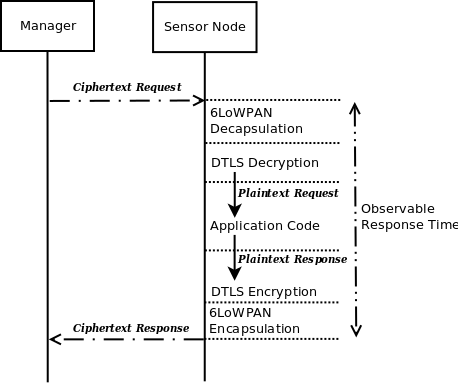
\includegraphics[width=0.8\textwidth]{fig/dtls_session.png}
	\caption{A Session with DTLS}
	\label{Fig: A Session with DTLS}
\end{figure*}

DTLS provides protection between only two Sensor Nodes in the network; thus the source and destination are consistent within a DTLS session. The 6LoWPAN encapsulation and decapsulation procedure are hence identical for all packets using the same DTLS session; therefore the time length of 6LoWPAN decapsulation and encapsulation in \Cref{Fig: A Session with DTLS} are considered to be constant.

Therefore in this section we put our interest in the timing of DTLS decryption/encryption and the execution time of application code.

\subsection{AES Timing} \label{tinydtls AES Timing}

tinydtls uses the OpenBSD optimised AES implementation. Its source code is available at:\\ 
\url{https://github.com/Salties/MyRepository/blob/master/tinydtls-0.8.2/aes/rijndael.c}

We applied the same tests as described in \Cref{Sec: AES Timing}. 

The average AES execution time is shown in \Cref{Tbl: tinydtls AES execution time estimation}.

\begin{table}[ht!]
	\center
	\begin{tabular}{|c|c|}
		\hline
		                        & CC2538 SW \\ \hline
		50 executions           & 160.07          \\ \hline
		100 executions          & 320.06          \\ \hline
		150 executions          & 480.05          \\ \hline
		200 executions          & 640.13          \\ \hline
		Ticks per executions    & 3.20            \\ \hline
		AES Execution Time (ms) & 0.098           \\ \hline
	\end{tabular}
	\caption{tinydtls AES execution time estimation}
	\label{Tbl: tinydtls AES execution time estimation}
\end{table}

The result of Fixed vs Random test is shown in \Cref{Tbl: Fixed vs Random test result for tinydtls AES execution time on CC2538}

\begin{table}[ht!]
	\center
	\begin{tabular}{|c|c|c|}
		\hline
		                         & Fixed       & Random      \\ \hline
		Sample Mean              & 640.28      & 640.25      \\ \hline
		Sample Standard Deviation & 0.49        & 0.53        \\ \hline
		t-score                  & \multicolumn{2}{c|}{1.32} \\ \hline
	\end{tabular}
	\caption{Fixed vs Random test result for tinydtls optimised AES execution time on CC2538. Executions per sample: $200$. Sample size: $1000$.}
	\label{Tbl: Fixed vs Random test result for tinydtls AES execution time on CC2538}
\end{table}

Applying the TVLA t-score threshold which is $4.5$, the results in \Cref{Tbl: Fixed vs Random test result for tinydtls AES execution time on CC2538} imply that the tinydtls optimised AES implementation has passed our test, i.e. no leakage is detected through the execution time of the tinydtls optimised AES implementation. 

The result is consistent with our expectation, as the implementation has no branch\footnote{The only branch in the source code is for AES-192 and AES-256, which are not used in the ciphersuites.} in the source code and is done with only statements of assignment, shift and XORs. The low sample standard deviation is also an evidence that supports our expectation that the AES implementation takes a nearly constant time.

The source code and data for our tinydtls AES timing experiments are available at: \\
\url{https://github.com/Salties/MyRepository/tree/master/experiments/dtlsaes} \\
and \\
\url{https://github.com/Salties/MyRepository/tree/master/experiments/dtlsaes/Data}

\subsection{Protocol Suite Processing Timing} \label{Protocol Suite Processing Time}

The observable response time in \Cref{Fig: A Session with DTLS}, , denotes as $t_R$, can be divided into two parts:

\begin{enumerate}
	\item Protocol suite processing time $t_P$. This part consists of the 6LoWPAN decapsulation / encapsulation and DTLS decryption / encryption in \Cref{Fig: A Session with DTLS}. $t_P$ is independent to the application. 
	\item Application code execution time $t_A$. It is one of the most interested information to the Adversary that could be exploited to learn information about the application data.
\end{enumerate}

Apparently we have
\begin{equation}
t_R = t_P + t_A
\end{equation}

One way to extract $t_A$ is to compute it by 
\begin{equation} \label{Eq: t_A}
t_A = t_R - t_P
\end{equation}

Practically, given a specific platform the value of $t_P$ is predictable, as it is independent to the upper layer application and the choices of different DTLS session key does not affect the timing as shown in \Cref{tinydtls AES Timing}. 

We estimated $t_P$ on CC2538 by an application where the Sensor Node replies to any Requests with a constant predefined value. A hint of the source code is shown in \Cref{nullapp}.

\lstinputlisting[label={nullapp}, captionpos=b, caption={Application code with negligible execution time}]{src/nullapp.c} 

Since no effective application code exists in this application, its $t_A$ can be considered negligible; hence the $t_R$ can be viewed as an approximation of $t_P$.

Avoid exceeding 802.15.4 MTU, the length of DTLS Payload can be ranged from $1$ byte to $47$ bytes. However in our setup, the Requests are forwarded by an Border Router and thus one byte is taken by the decompressed Hop Limit in IPv6 Header; therefore the the length of DTLS Payload in our Requests is ranged from $1$ byte to $46$ bytes.

\Cref{Fig: Example histograms of protocol suite processing time on CC2538 with DTLS} shows two example histograms of part of our result. We denote $|Req|$ and $|Res|$ as the length in bytes of the DTLS Payload in Requests and Responses respectively.

\begin{figure}[ht!]
	\center
	\begin{subfigure}{.45\textwidth}
	\center
	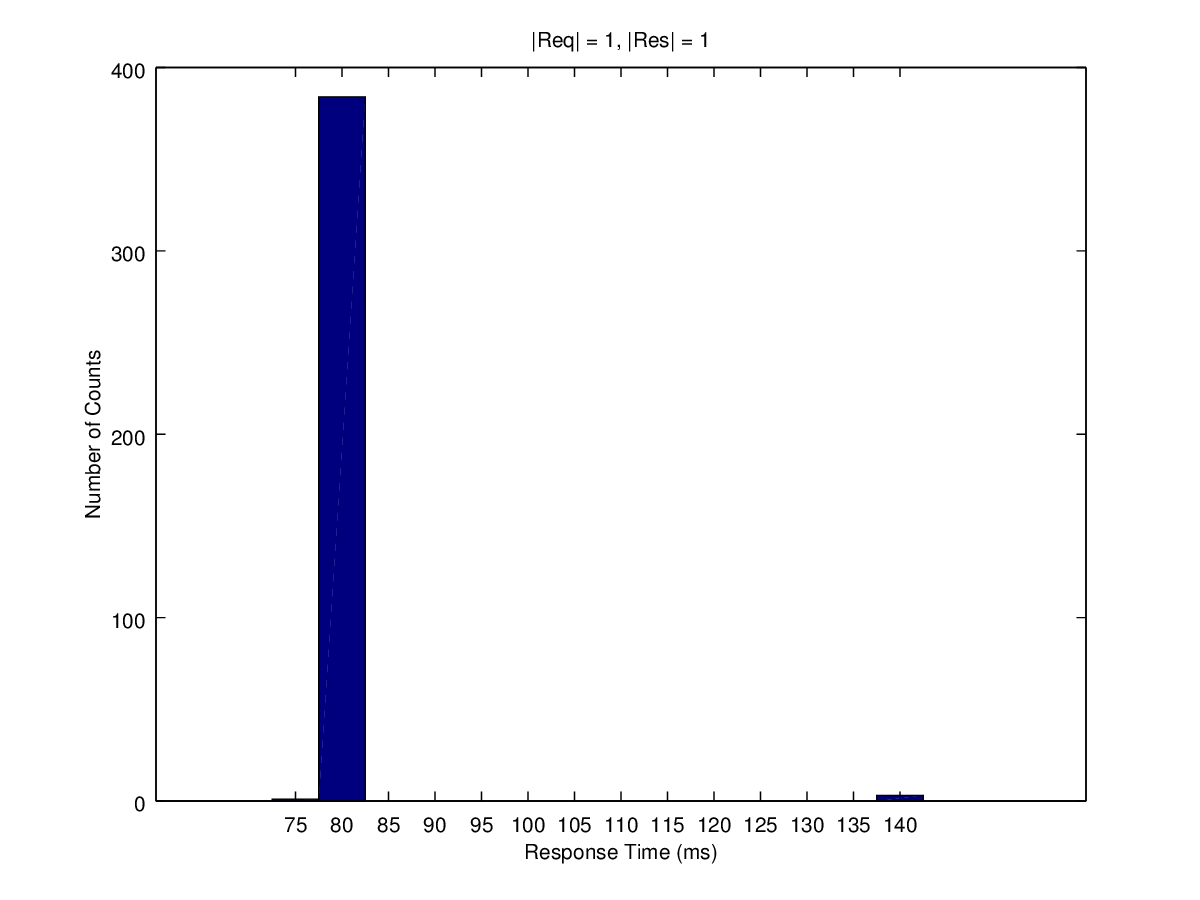
\includegraphics[width=\linewidth]{fig/dtlstimehist_min.png}
	\end{subfigure}
	\begin{subfigure}{.45\textwidth}
	\center
	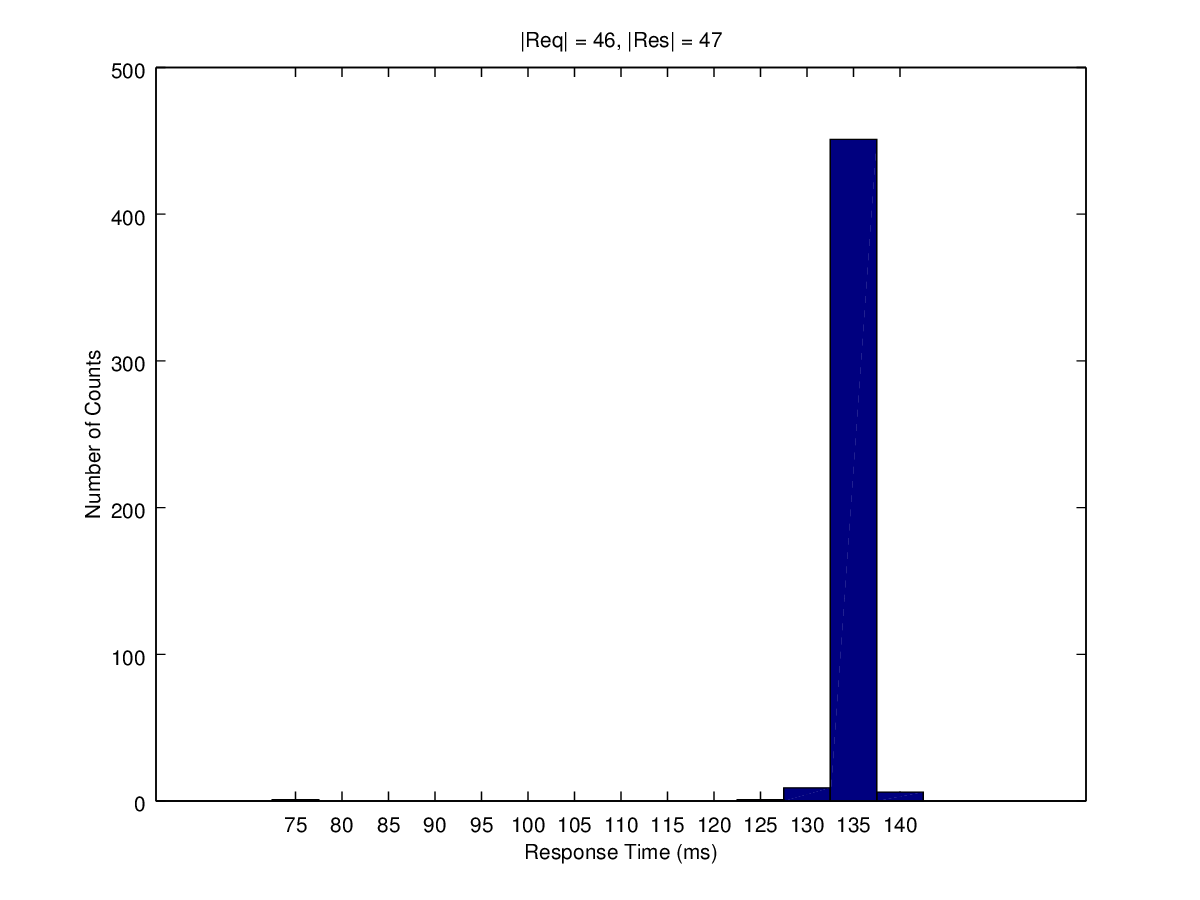
\includegraphics[width=\linewidth]{fig/dtlstimehist_max.png}
	\end{subfigure}
	\caption{Example histograms of protocol suite processing time on CC2538 with DTLS}
	\label{Fig: Example histograms of protocol suite processing time on CC2538 with DTLS}
\end{figure}

Similar to the ECHO response time,$t_R$ in the samples also appeared to densely clustered near a specific value while a few are drifted away; hence we use the sample median to characterise $t_R$ in our experiments. Medians of the examples in \Cref{Fig: Example histograms of protocol suite processing time on CC2538 with DTLS} are summarised in \Cref{Tbl: Median of response times in examples}. It is clear that when $|Req|$ and $|Res|$ are at their maximum value, $t_R$ is significantly longer comparing to $Req$ and $Res$ at their minimum value.
 
\begin{table}
	\center
	\begin{tabular}{|c|c|c|}
		\hline
		 				&($|Req| = 1$, $|Res| = 1$) 	& ($|Req| = 46$, $|Res| = 47$) 	\\ \hline
		 Sample Median	&79.712 ms                  			& 132.740 ms                   			\\ \hline
	\end{tabular}

	\caption{Medians of response time in the examples of \Cref{Fig: Example histograms of protocol suite processing time on CC2538 with DTLS}}
	\label{Tbl: Median of response times in examples}
\end{table}

We measured $t_R$ with different combinations of $|Req|$ and $|Res|$. The results are shown in \Cref{Fig: Protocol suite processing time on CC2538 with DTLS}.

\begin{figure}[ht!]
	\center
	\begin{subfigure}{0.45\linewidth}
	\center
	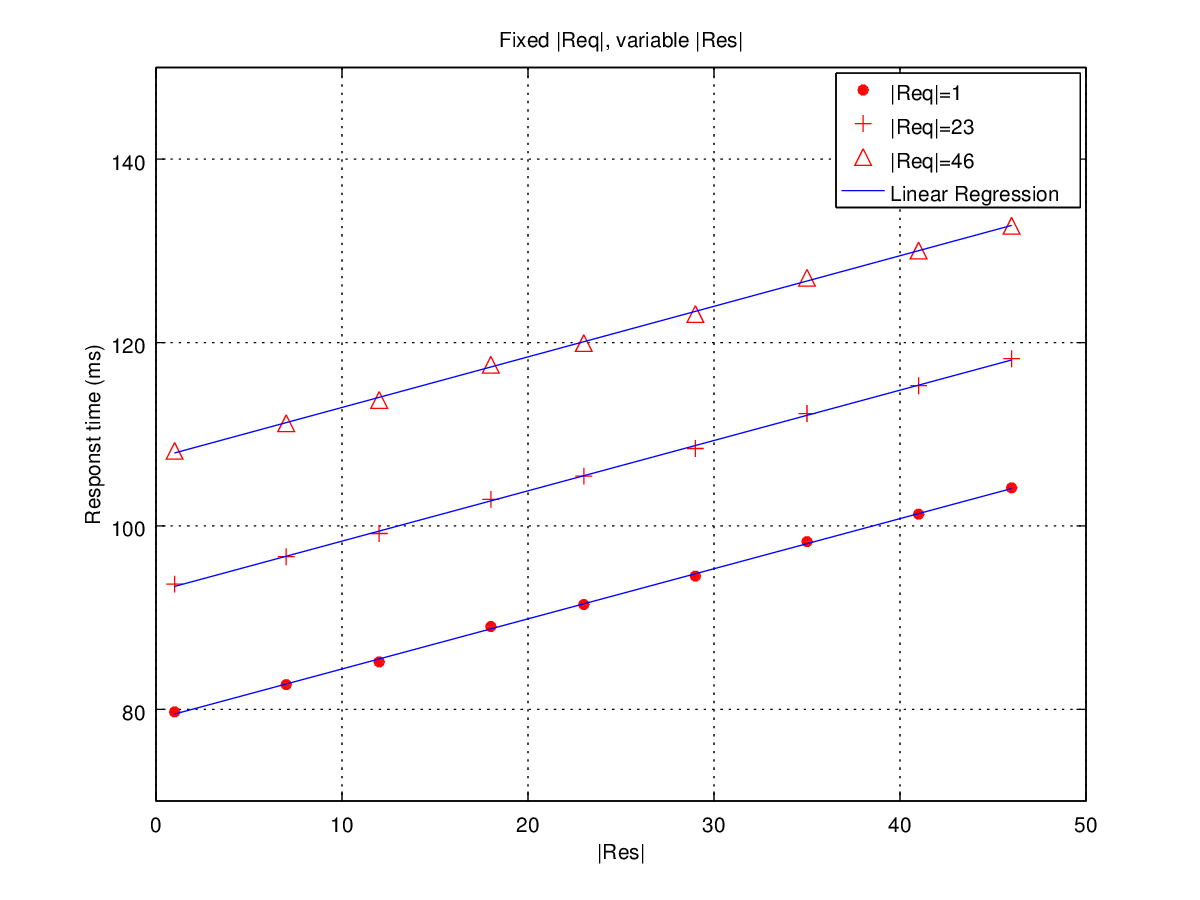
\includegraphics[width=\textwidth]{fig/dtlstime_fixed_req.png}
	\subcaption{Response time($t_R$) with $|Req| \in \{1, 23, 46\}$}
	\end{subfigure}
	\begin{subfigure}{0.45\linewidth}
	\center
	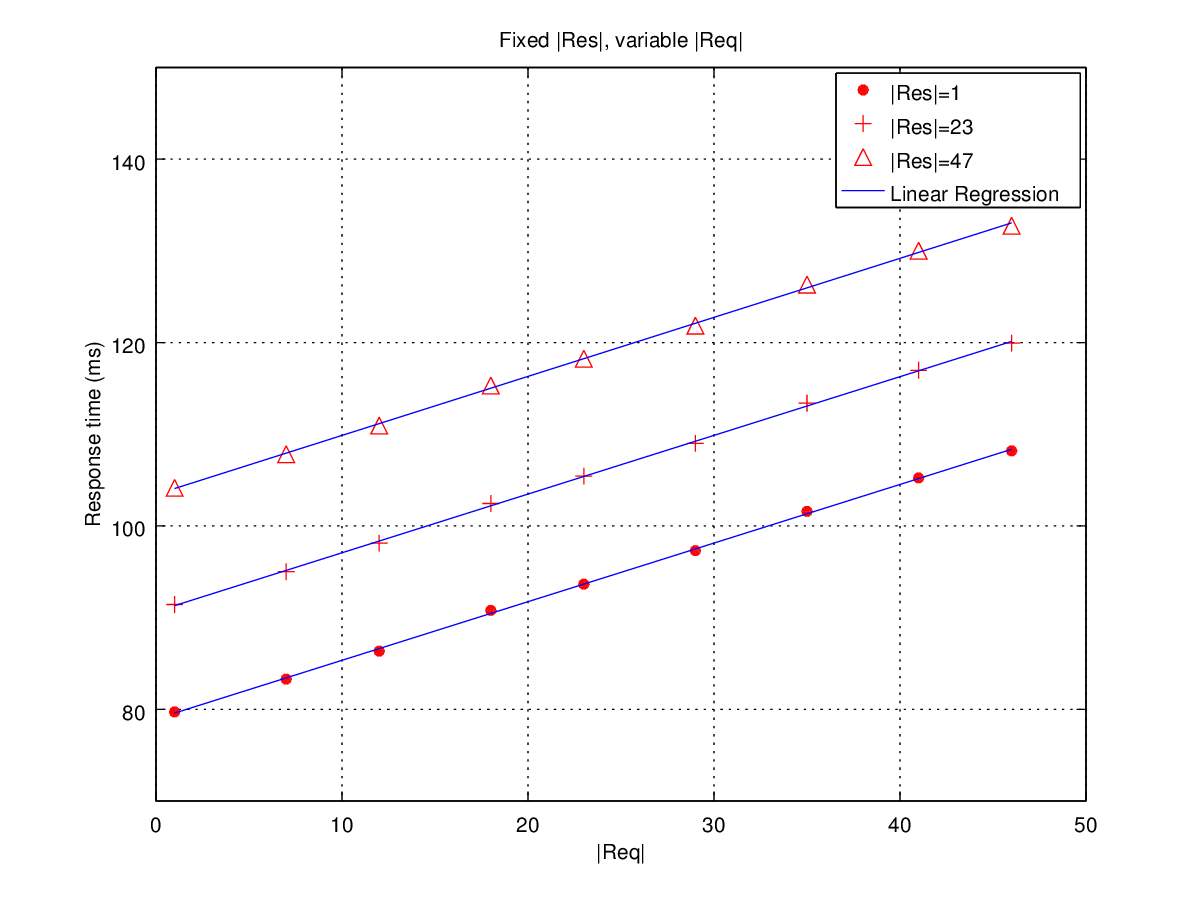
\includegraphics[width=\textwidth]{fig/dtlstime_fixed_res.png}
	\subcaption{Response time($t_R$) with $|Res| \in \{1, 23, 46\}$}
	\end{subfigure}
	\caption{Protocol suite processing time on CC2538 with DTLS}
	\label{Fig: Protocol suite processing time on CC2538 with DTLS}
\end{figure}

The results in \Cref{Fig: Protocol suite processing time on CC2538 with DTLS} suggest that $|Req|$ and $|Res|$ might both be linear to the $t_R$ on CC2538. Assume $t_R$ is in the form of:
\begin{equation} \label{Eq: tR est}
	t_R = b_0 + b_1|Req| + b_2|Res|
\end{equation}

Applying multiple linear regression using least squares fit, we have an estimation of $t_R$ (in ms) for CC2538:

\begin{equation}
	\hat{t}_R = 78.388 + 0.538|Req| + 0.638|Res|
	\label{Eq: t_R estimation}
\end{equation}

The $R^2$ for the extimation of \Cref{Eq: t_R estimation} is $0.9997$, which is consistent to our intuition of \Cref{Fig: Protocol suite processing time on CC2538 with DTLS}.

Since $t_A$ in this application is negligible, we therefore approximate $t_P$ by $t_R$ for CC2538:
\begin{equation} \label{Eq: CC2538tP}
	\hat{t}_P \approx \hat{t}_R = 78.388 + 0.538|Req| + 0.638|Res|
\end{equation}

In the WSN scenario described in \Cref{Fig: Experiment Setup}, $t_R$ is directly observable from the captured traffic. Given the estimation $\hat{t}_P$, we can further estimate the the application execution time by substituting $t_P$ in \Cref{Eq: t_A} by $\hat{t}_P$:
\begin{equation} \label{Eq: hattA}
	\hat{t}_A = t_R - \hat{t}_P
\end{equation}

We discuss more details of this estimation in \Cref{App code timing}.

The source code and data for our protocol suite processing timing experiments are available at: \\
\url{https://github.com/Salties/MyRepository/tree/master/experiments/dtlstime} \\
and \\
\url{https://github.com/Salties/MyRepository/tree/master/experiments/dtlstims/Data}

\subsection{Application Code Timing} \label{App code timing}

\Cref{Eq: hattA} provides a method to estimate the application code execution time on a Sensor  Node. To test this method, we used an application that repeatedly invokes the Contiki system random number generator according to the data in the Request, and replies the execution time as the Response. The random number generator is selected arbitrary to provide some payload for $t_A$. In real world applications, the random number generator will be replaced by actual application code, such as reading a sensor or actual data processing. The code of our application is hinted by \Cref{apptime}.

\lstinputlisting[label={apptime}, captionpos=b, caption={Code for application code timing}]{src/dtlsapptime.c} 

We tested \Cref{Eq: t_A} with \Cref{apptime} on CC2538 with different execution time induced by different Request data, with $t_P$ estimated by \Cref{Eq: CC2538tP}. 

We denote the actual execution time returned in the Response as $t_A$ and the estimated execution time as $\hat{t}_A$. We further denote their absolute and relative approximation error as $\epsilon$ and $\mu$ respectively, where:
\begin{eqnarray}
	\begin{aligned}
		\epsilon	&= |t_A - \hat{t}_A| \\
		\mu 	&= \epsilon / |t_A|
	\end{aligned}
\end{eqnarray}

For clarity, we arbitrarily divide our data into three groups:
\begin{itemize}
	\item Low $t_A$, for $t_A < 1.5$ ms.
	\item Medium $t_A$, for $t_A \in [1.5, 25)$ ms.
	\item High $t_A$, for $t_A \geq 25$ ms.
\end{itemize}

The source code and data for our application code timing estimation experiments are available at: \\
\url{https://github.com/Salties/MyRepository/tree/master/experiments/dtlsapptime} \\
and \\
\url{https://github.com/Salties/MyRepository/tree/master/experiments/dtlsapptime/Data/varrnd}

\subsubsection{Low Execution Time}

The result for  low $t_A$ ($<1.5$ ms) is shown in \Cref{Fig: Estimation for low tA}.

\begin{figure}[ht!]
	\center
	\begin{subfigure}{0.6\linewidth}
	\center
	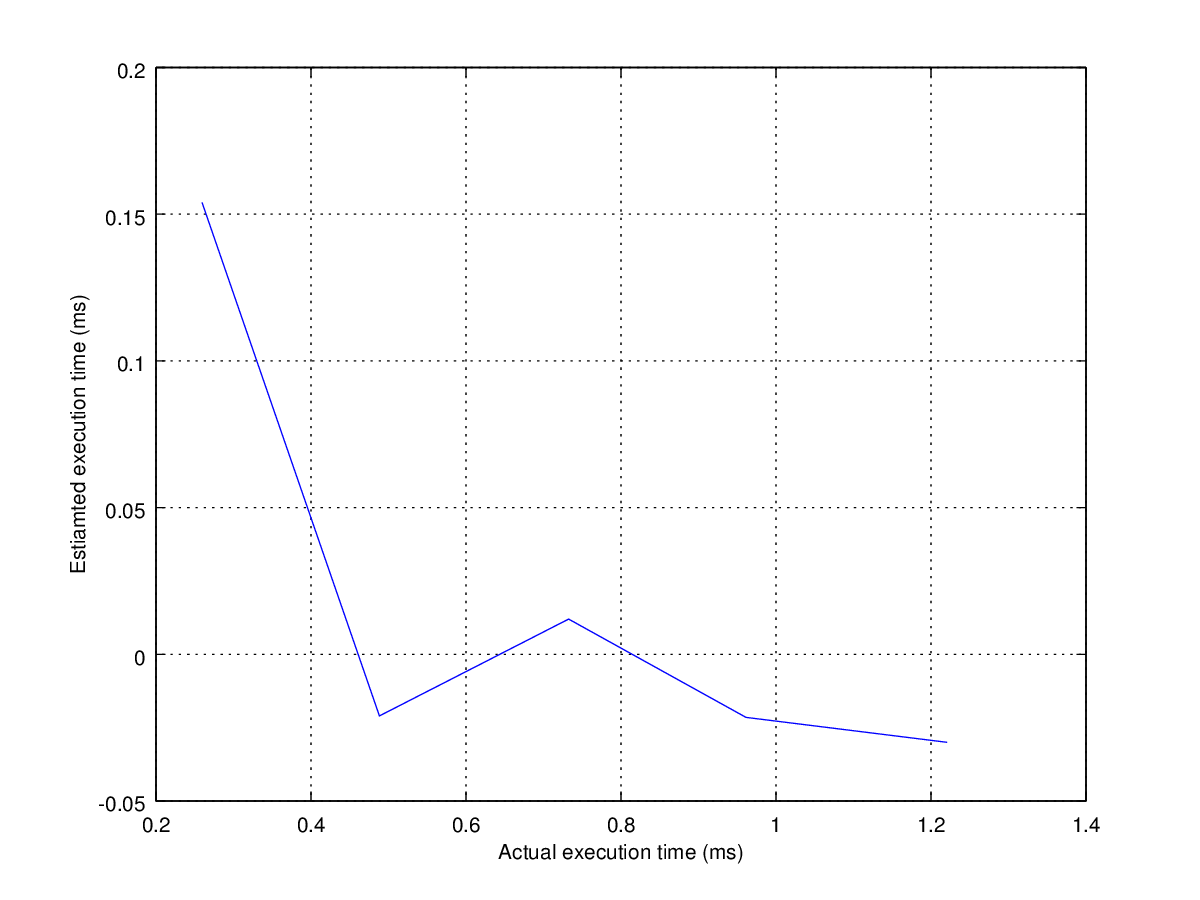
\includegraphics[width=\linewidth]{fig/lowtaest.png}
	\subcaption{Estimated execution time $\hat{t}_A$}
	\end{subfigure}
	\begin{subfigure}{0.45\linewidth}
	\center
	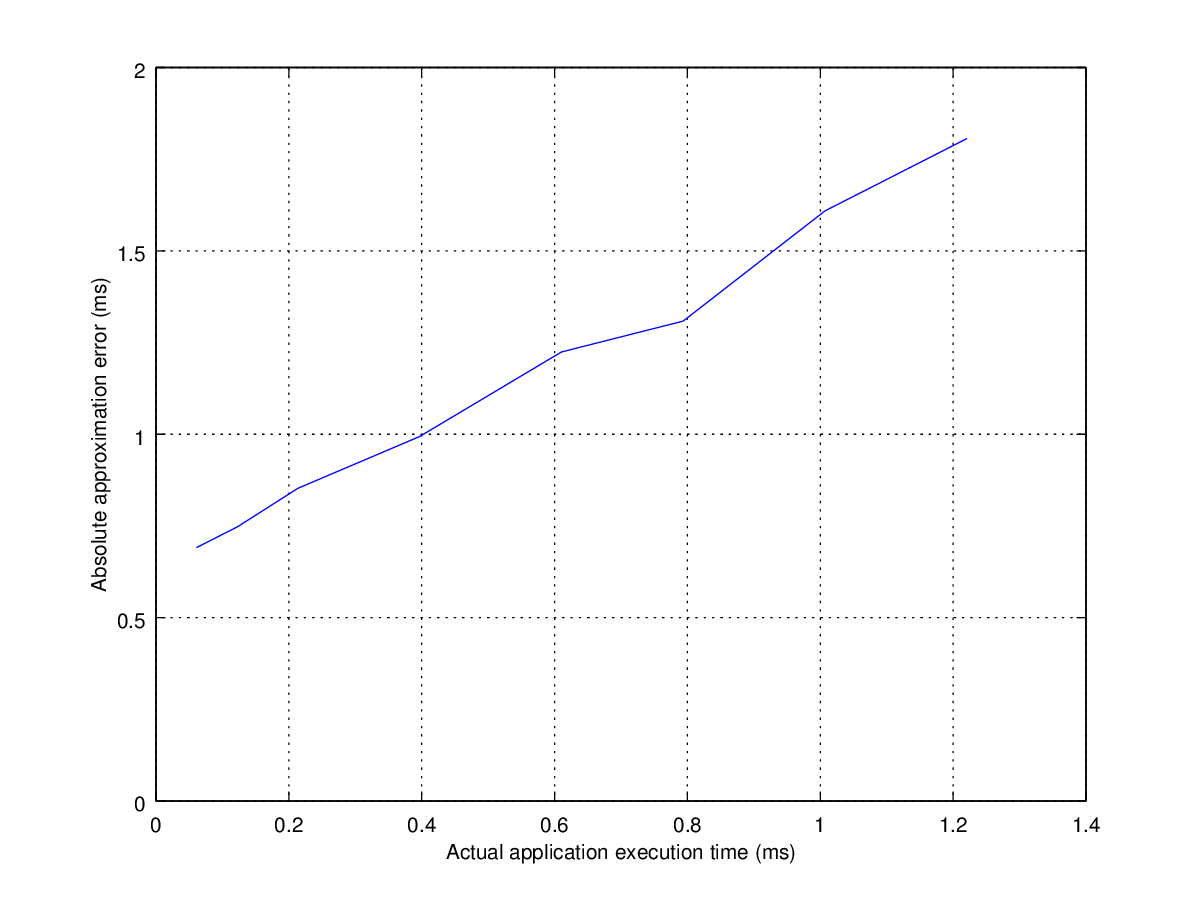
\includegraphics[width=\linewidth]{fig/lowabstaerr.png}
	\subcaption{Absolute approximation error $\epsilon$}
	\end{subfigure}
	\begin{subfigure}{0.45\linewidth}
	\center
	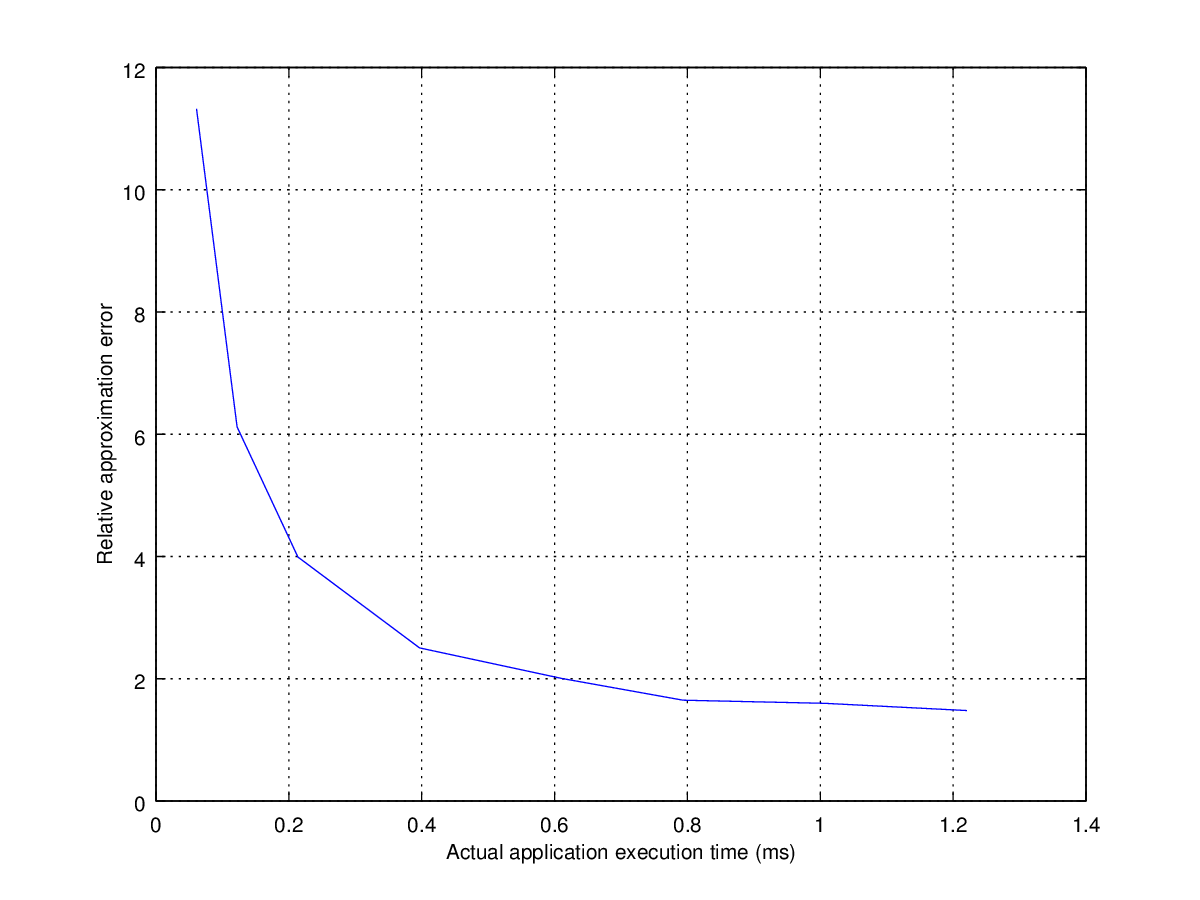
\includegraphics[width=\linewidth]{fig/lowrtvtaerr.png}
	\subcaption{Relative approximation error $\mu$}
	\end{subfigure}
	\caption{Estimation for low $t_A$($<1.5$ms) on CC2538}
	\label{Fig: Estimation for low tA}
\end{figure}

The result in \Cref{Fig: Estimation for low tA} indicates that the estimation totally failed at low $t_A$ such that even negative values are estimated. We consider this is caused by the fact that at such level $t_A$ is negligible and is dominated by the systematic noise. $\epsilon$ increases nearly linearly with $t_A$, whilst $\mu$ indicates that the estimation does not make much sense at this level of $t_A$.

\subsubsection{Medium Execution Time}

For $t_A$ with medium values ($t_A \in[1.5, 100)$ ms), the results are shown in \Cref{Fig: Estimation for medium tA}.

\begin{figure}[ht!]
	\center
	\begin{subfigure}{0.6\linewidth}
	\center
	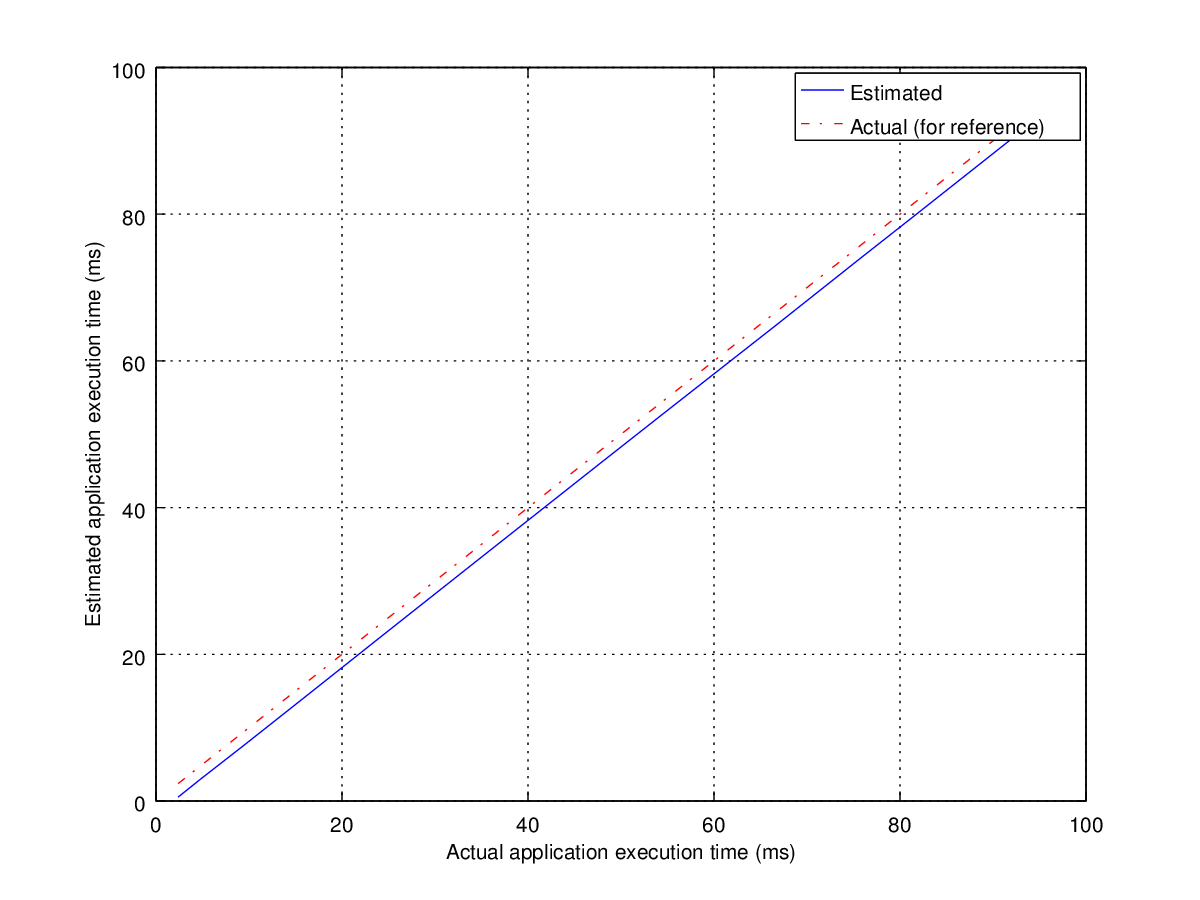
\includegraphics[width=\linewidth]{fig/midtaest.png}
	\subcaption{Estimated execution time $\hat{t}_A$}
	\end{subfigure}
	\begin{subfigure}{0.45\linewidth}
	\center
	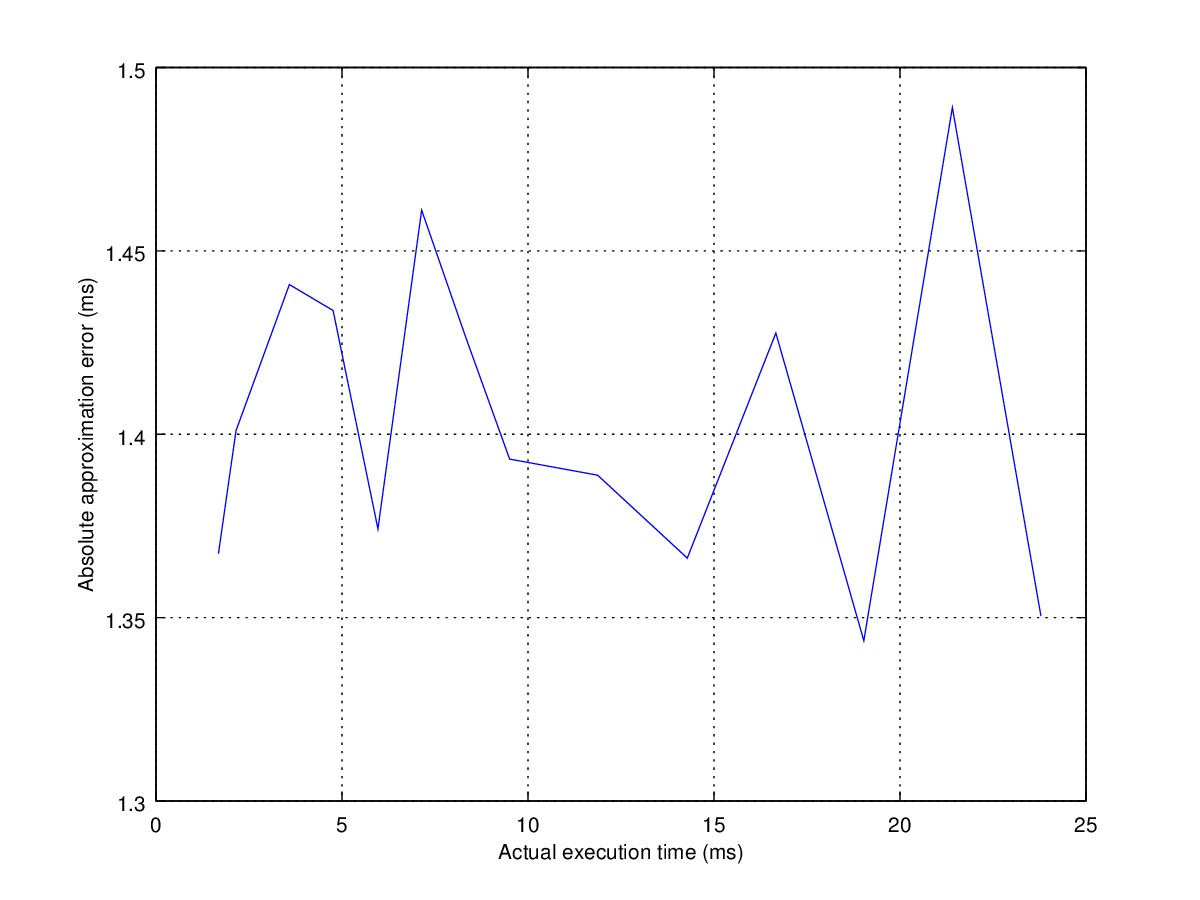
\includegraphics[width=\linewidth]{fig/midabstaerr.png}
	\subcaption{Absolute approximation error $\epsilon$}
	\end{subfigure}
	\begin{subfigure}{0.45\linewidth}
	\center
	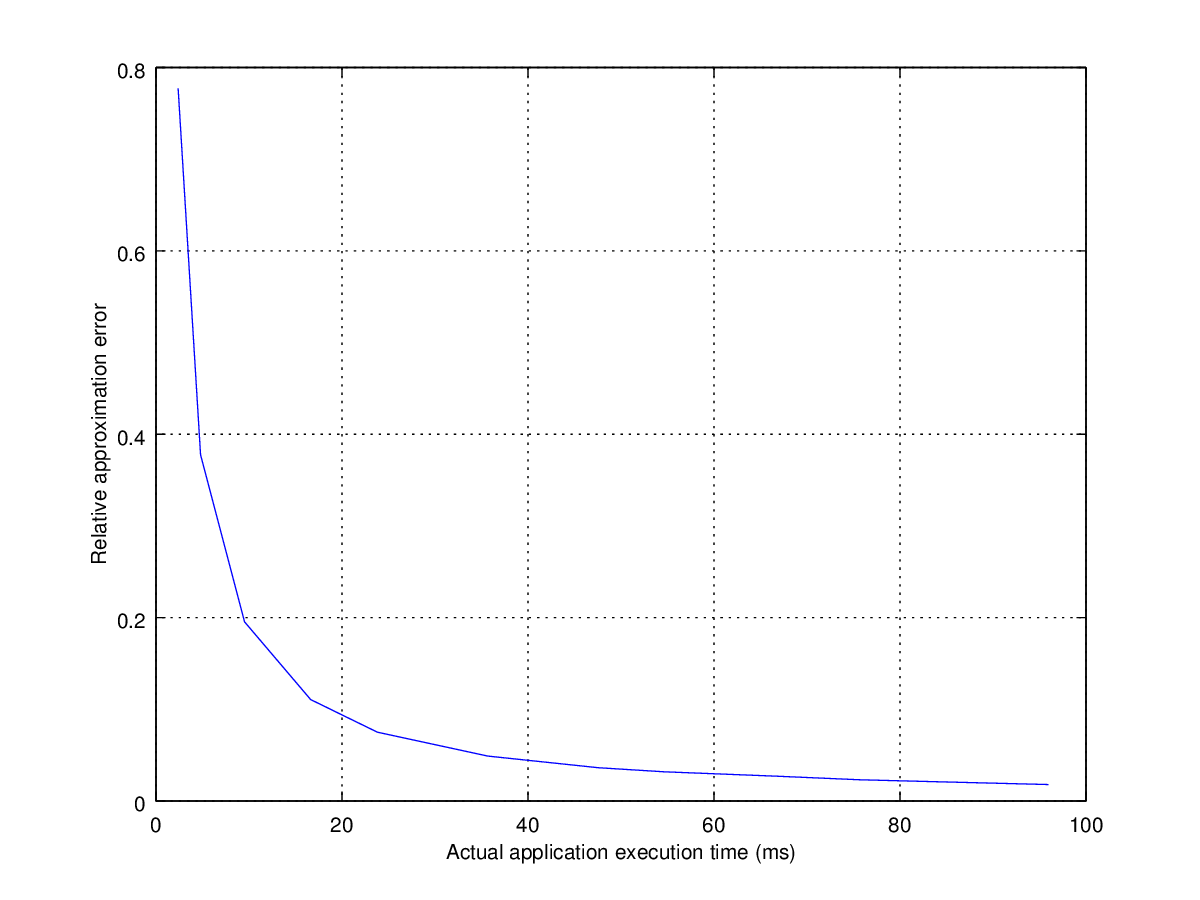
\includegraphics[width=\linewidth]{fig/midrtvtaerr.png}
	\subcaption{Relative approximation error $\mu$}
	\end{subfigure}
	\caption{Estimation for medium $t_A$($[1.5,100)$ ms) on CC2538}
	\label{Fig: Estimation for medium tA}
\end{figure}

$\hat{t}_A$ increase nearly linearly with $t_A$ in \Cref{Fig: Estimation for medium tA}. However, we realised that our estimations are strictly beneath the actual value. The $\epsilon$ appears to be random with medium $t_A$,  ranging $[1.34, 1.49]$ ms.  The sample mean and standard deviation for $\epsilon$ are $1.405$ and $0.043$ ms respectively in these experiments. Due to the narrow range of $\epsilon$, $\mu$ decreases inverse proportionally as $t_A$ increases.

Applying least squares fitting, we have an estimation of medium $t_A$:
\begin{equation}
	t_A = 1.412 + 0.999\hat{t}_A 
\end{equation}

with $R^2=1.000$, which indicates that $\hat{t}_A$ is almost perfectly linear to $t_A$. 

The result suggests that for medium $t_A$, the accuracy of estimation increases as $t_A$ increases. 

\subsubsection{High Execution Time}

Further increasing $t_A$, we have the result for high $t_A$ ($\geq 25$ ms), shown in \Cref{Fig: Estimation for high tA}.

\begin{figure}[ht!]
	\center
	\begin{subfigure}{0.6\linewidth}
	\center
	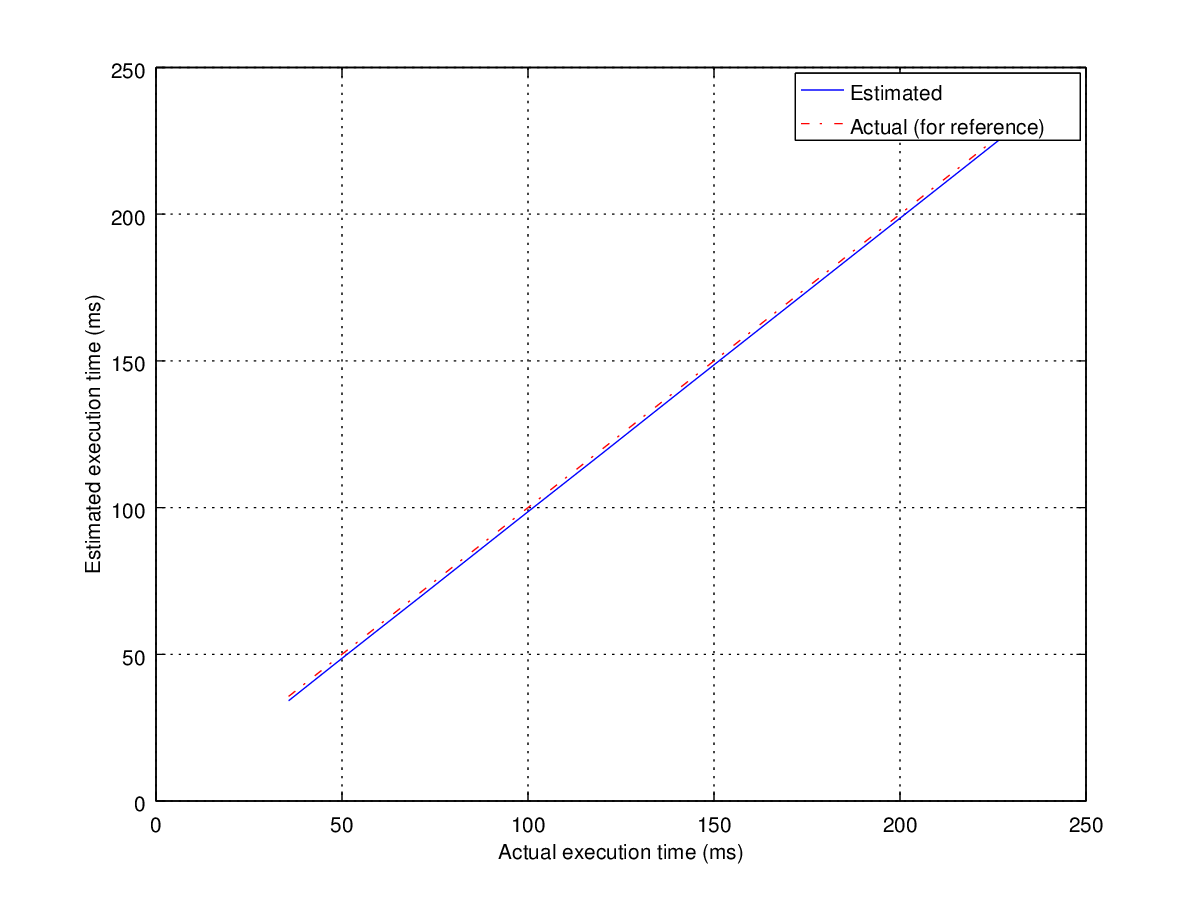
\includegraphics[width=\linewidth]{fig/hightaest.png}
	\subcaption{Estimated execution time $\hat{t}_A$}
	\end{subfigure}
	\begin{subfigure}{0.45\linewidth}
	\center
	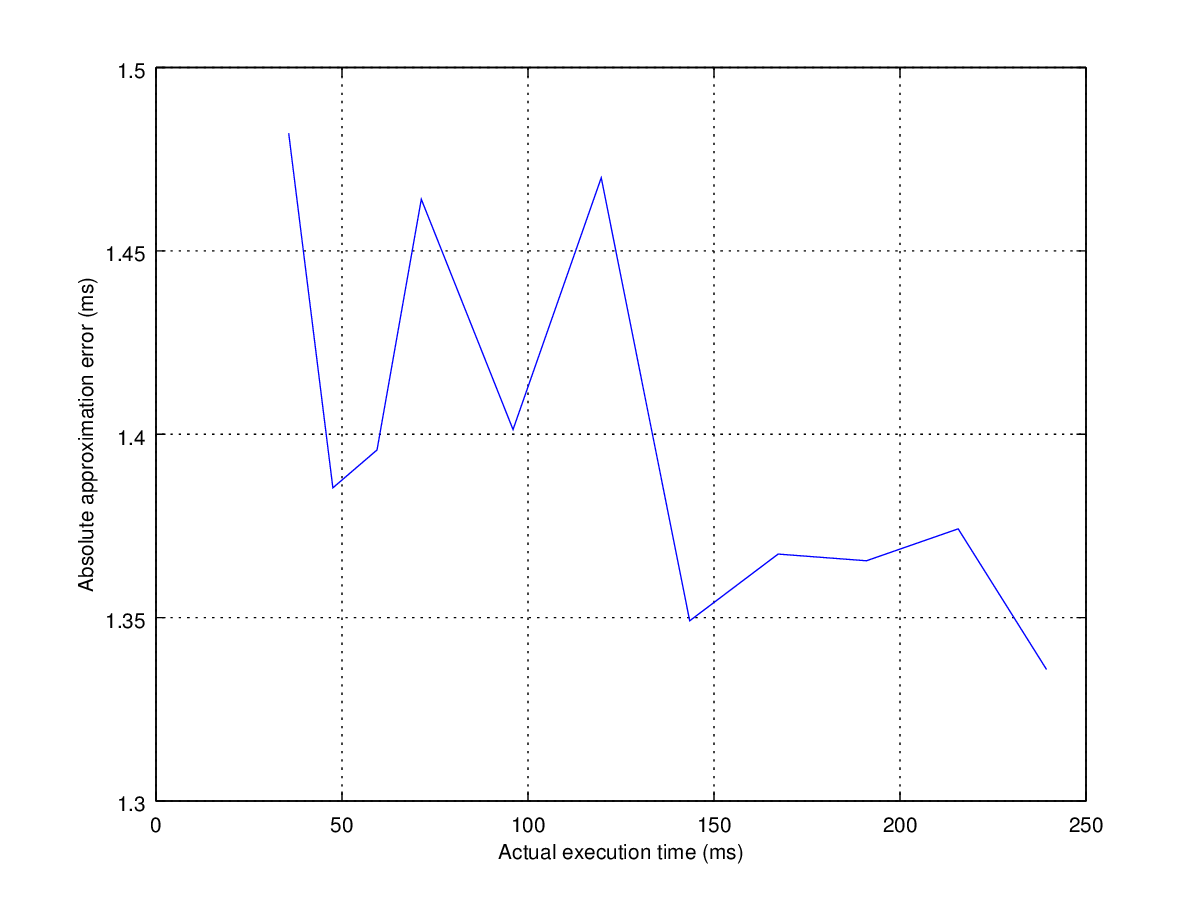
\includegraphics[width=\linewidth]{fig/highabstaerr.png}
	\subcaption{Absolute approximation error $\epsilon$}
	\end{subfigure}
	\begin{subfigure}{0.45\linewidth}
	\center
	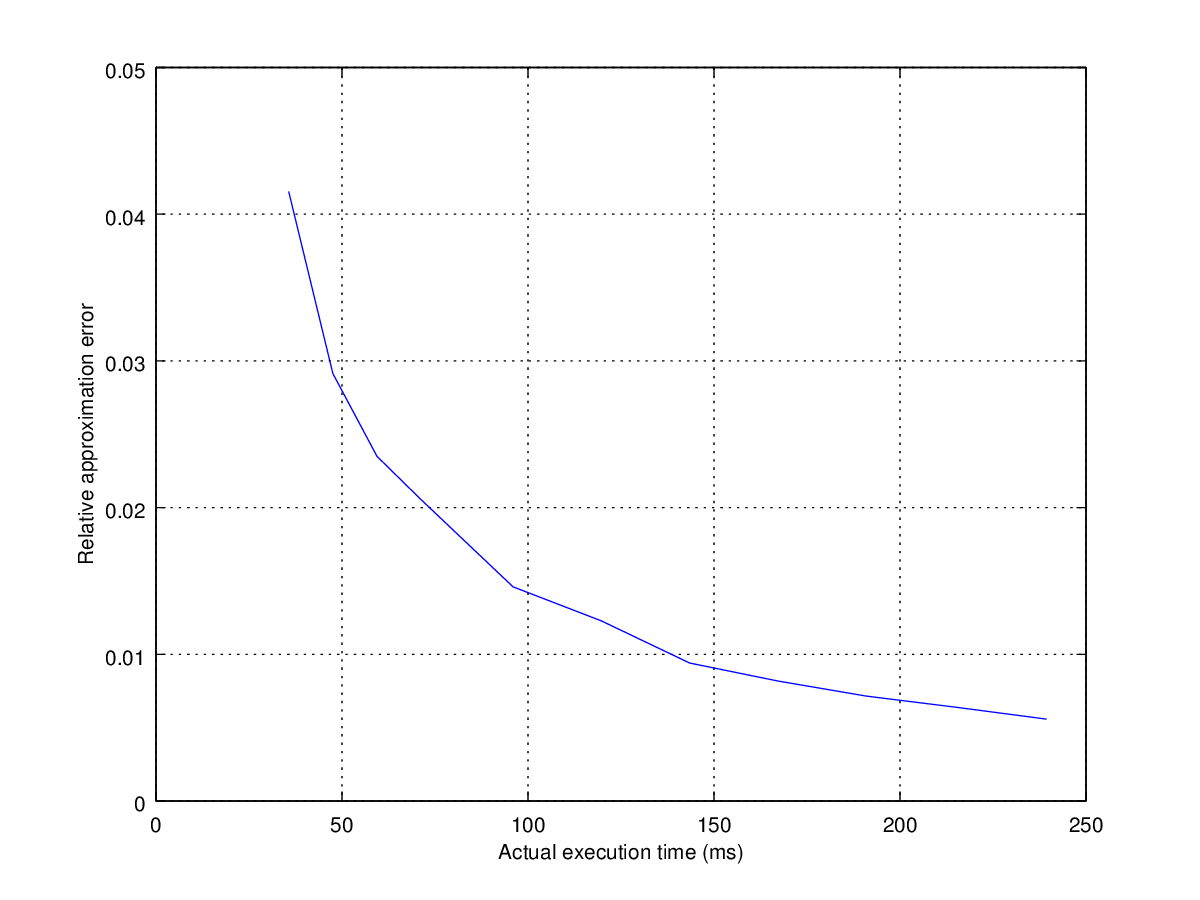
\includegraphics[width=\linewidth]{fig/highrtvtaerr.png}
	\subcaption{Relative approximation error $\mu$}
	\end{subfigure}
	\caption{Estimation for high $t_A$($\geq 100$ ms) on CC2538}
	\label{Fig: Estimation for high tA}
\end{figure}

The result in \Cref{Fig: Estimation for high tA} is similar to the result of medium $t_A$ such that $\hat{t}_A$ is almost linear to $t_A$ that nearly overlapped. The least square estimation of high $t_A$ group is:
\begin{equation}
	t_A = 1.459 + 1.000\hat{t}_A
\end{equation}

where $R^2 = 1.000$. 

The absolute approximation error $\epsilon$ in high $t_A$ has sample mean and standard deviation of $1.399$ and $0.051$ respectively, ranging in $[1.34, 1.48]$ ms.

The relative approximation error $\mu$ further decreases in this group, down to $0.041$  for $t_A = 35.8$ ms and $0.009$ for $t_A = 143.5$ ms


\subsection{Errors}

The absolute approximation error $\epsilon$ is defined to be signledness. We further define the signed approximation error :
\begin{equation} \label{Eq: e}
e = t_A - \hat{t}_A
\end{equation}

We show the overall signed approximation error among of all $t_A$ we tested in \Cref{Fig: Overall approximation error}.

\begin{figure}[ht!]
	\center
	\begin{subfigure}{0.45\linewidth}
		\center
		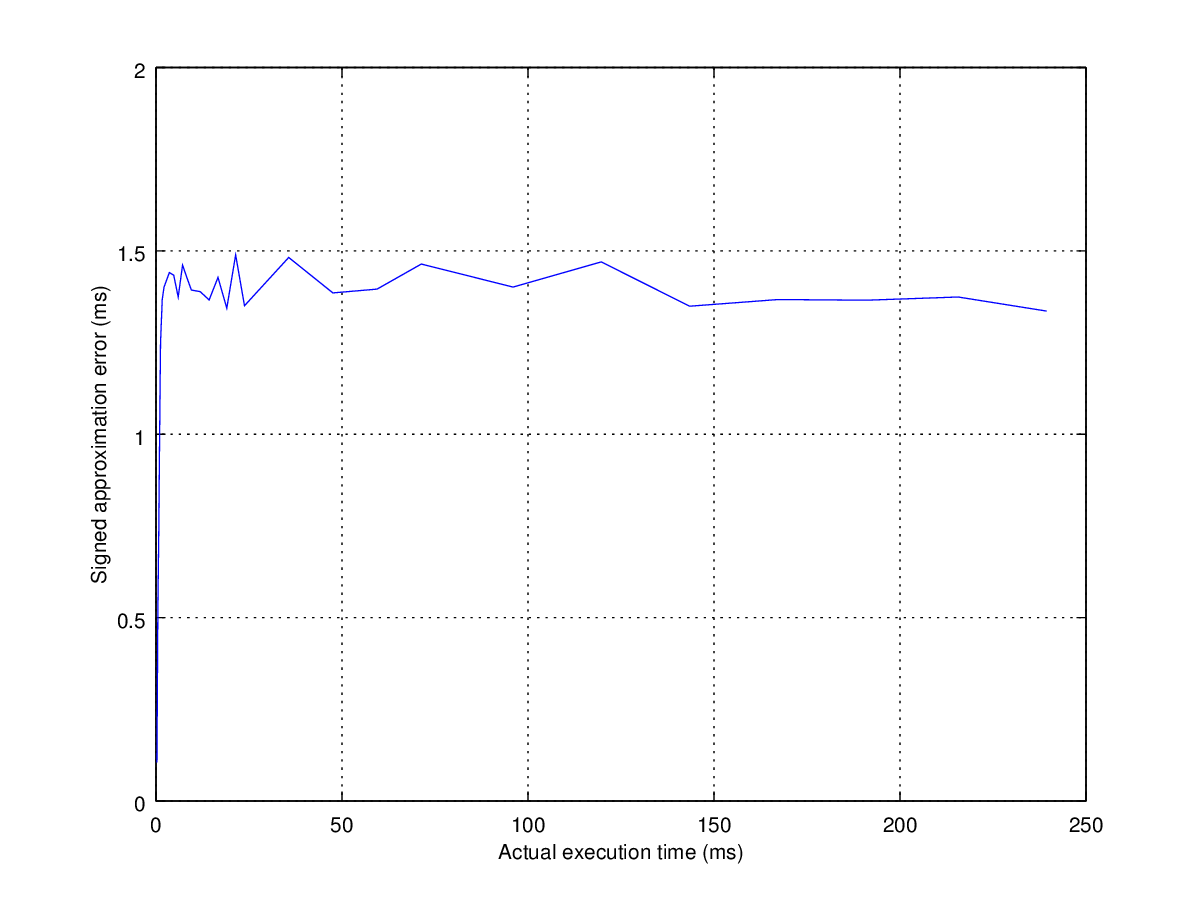
\includegraphics[width=1\linewidth]{fig/esterr.png}
		\subcaption{Signed approximation error ($e$)}
	\end{subfigure}
	\begin{subfigure}{0.45\linewidth}
		\center
		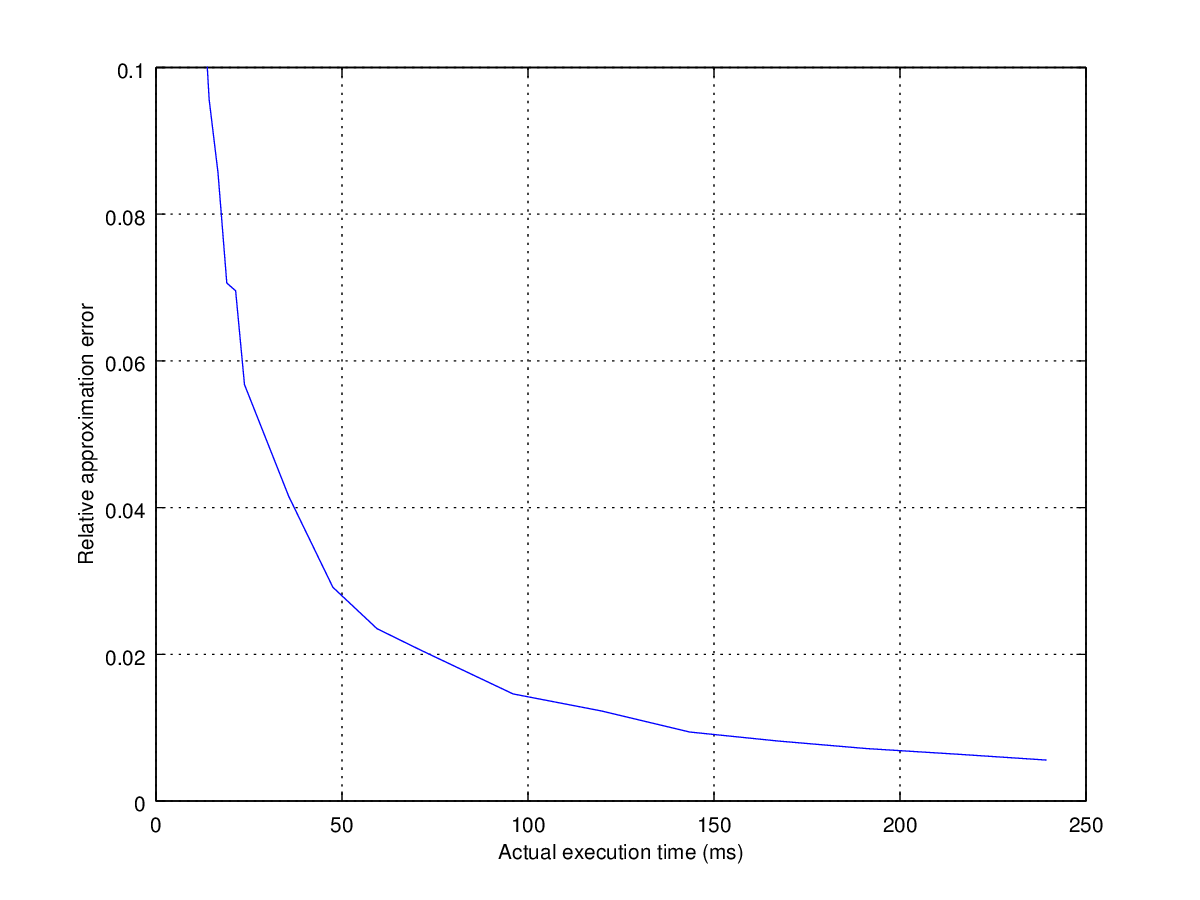
\includegraphics[width=\linewidth]{fig/rtvesterr.png}
		\subcaption{Relative estimation error ($\mu$), for $< 0.1$}
	\end{subfigure}
	\caption{Overall approximation error}
	\label{Fig: Overall approximation error}
\end{figure}

The result suggests that $e$ dramatically increases at low $t_A$ but quickly converges to [1.34, 1.49] ms at medium($[1.5, 25)$ ms) and high $t_A$ ($>25$ ms). From a practical aspect, it would be reasonable to simply approximate the negligible low $t_A$ as $0$ ms. Also the positive errors indicates that $t_A$ is generally underestimated.

For the converged $e$, i.e. when $t_A > 1.5$ ms, the sample mean and standard deviation of $e$ are $1.402$ ms and $0.046$ ms respectively. The result of Shapiro-Wilk nomality test on $e$ in our data suggests that $e$ is likely to be normally  distributed.

Considering the fact that the sample mean of $e$ is much greater than its standard deviation, we suppose it is dominated by a systematic error. The potential cause of the error we considered are:
\begin{itemize}
	\item Implicit affection of application code.
	\item Error in estimation of $t_P$.
	\item Error in measurement of $t_A$.
\end{itemize}

Due to practical reason, the last cause is difficult to verify; hence we focus on the implicit affection of application code and error in estimation of $t_P$.

\subsubsection{Affection of application code} \label{Affection of application code}

As a comparison, we replace the random number generator by Contiki software AES encryption call and then computed the error. The result is shown in \Cref{Fig: Overall estimation error for AES replacement}.

\begin{figure}[ht!]
	\center
	\begin{subfigure}{0.45\linewidth}
		\center
		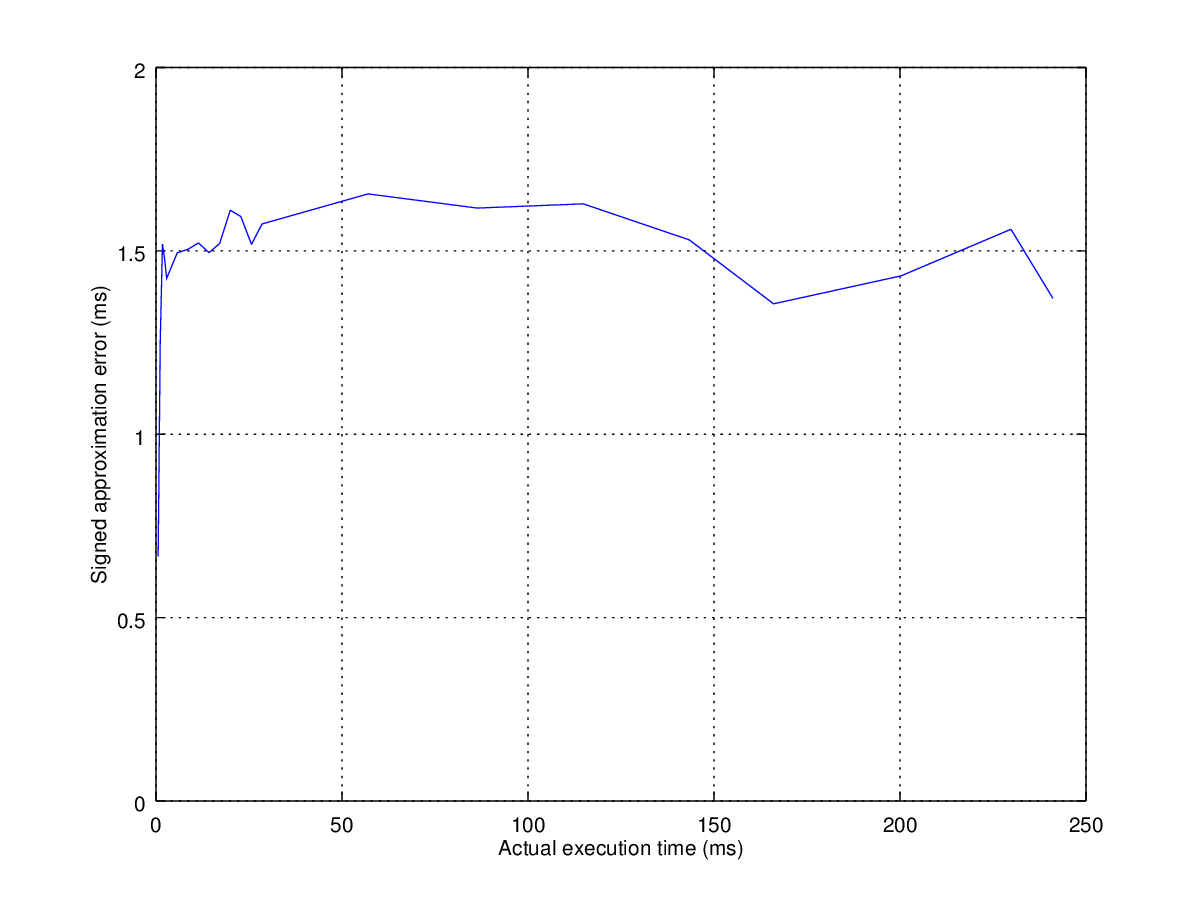
\includegraphics[width=1\linewidth]{fig/esterraes.png}
		\subcaption{Signed approximation error ($e$)}
	\end{subfigure}
	\begin{subfigure}{0.45\linewidth}
		\center
		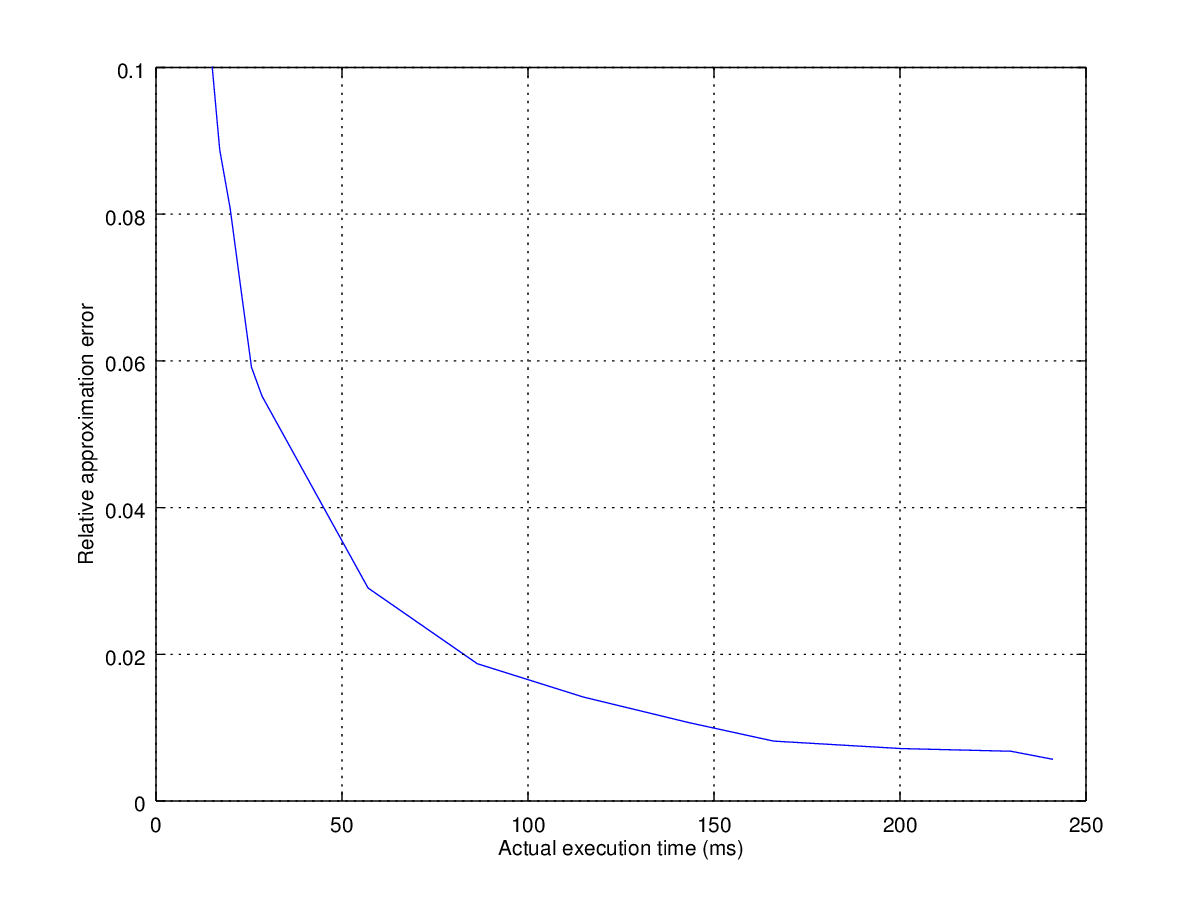
\includegraphics[width=\linewidth]{fig/rtvesterraes.png}
		\subcaption{Relative estimation error ($\mu$), for $< 0.1$}
	\end{subfigure}
	\caption{Overall approximation error for AES replacement}
	\label{Fig: Overall estimation error for AES replacement}
\end{figure}

We denote $e_{RND}$ and $e_{AES}$ to be the singed approximation errors in the original application with random number call, i.e. the application showed in \Cref{apptime}, and its AES encryption replacement. Intuitively, $e_A$ showed some similar characteristics of $e_R$:

\begin{itemize}
	\item They both dramatically increases at low $t_A$, then converges into some range at medium and high $t_A$.
	\item The relative approximation error $\mu$ decreases nearly inverse proportionally, reaching $<0.1$ at $25$ ms.
\end{itemize}

The converged sample mean and standard deviation for $e_A$ are $1.520$ ms and $0.082$ ms respectively. Again using Shapiro-Wilk normality test, the result indicates that $e_A$ is also likely to be normally distributed.

We summarise the statistical features of $e_R$ and $e_A$ in \Cref{Tbl: Statistical features of eR and eA}.

\begin{table}
	\center
	\begin{tabular}{|c|c|c|}
	\hline
	      & Sample Mean (ms) & Sample Standard Deviation (ms) \\ \hline
	$e_{RND}$ & 1.402            & 0.046                          \\ \hline
	$e_{AES}$ & 1.520            & 0.082                          \\ \hline
	\end{tabular}
	\caption{Statistical features of $e_{RND}$ and $e_{AES}$}
	\label{Tbl: Statistical features of eR and eA}
\end{table}

Using two sample t-test on $e_R$ and $e_A$, the result shows that they are unlikely to have the same mean; therefore we conclude that the replacement of AES did affect the error in our estimations. 

In another word, the results implies that the application code could potentially The mechanism of such affection is not clear so far; thus such error would be difficult to quantify as it is directly related the specific application code. We leave the cause of this error as an open question in this report. However in practice, we would argue that such error can be mitigated as $t_A$ increases, as depicted by the relative approximation errors in \Cref{Fig: Overall approximation error} and \Cref{Fig: Overall estimation error for AES replacement}.

\subsubsection{Error in estimation of protocol suite processing time}

Substituting \Cref{Eq: t_A} and \Cref{Eq: hattA} into \Cref{Eq: e}, we have:

\begin{equation}\label{Eq: tP error}
	\begin{aligned}
		e &= t_A - \hat{t}_A = (t_R - t_P) - (t_R - \hat{t}_P) = \hat{t}_P - t_P\\
		t_P &= \hat{t}_P - e
	\end{aligned}
\end{equation}

Our estimation in \Cref{Eq: CC2538tP} solely depends on$|Req|$ and $|Res|$, while our experiments in \Cref{Affection of application code} suggests that $e$ has dependency to the application code. These combined together implies that given a fixed estimation $\hat{t}_P$, the protocol suite processing time $t_P$ can vary due to different application code.

We therefore conducted similar experiments as in \Cref{Protocol Suite Processing Time}, with $t_A$ adjusted to a fixed amount of time using Contiki random number generator call. \Cref{Fig: e by len} shows the result of how $e$ is affected by $|Req|$ and $|Res|$, on $t_A$ adjusted to $5$ ms and $25$ ms respectively.

\begin{figure}[ht!]
	\center
	\begin{subfigure}{0.45\linewidth}
		\center
		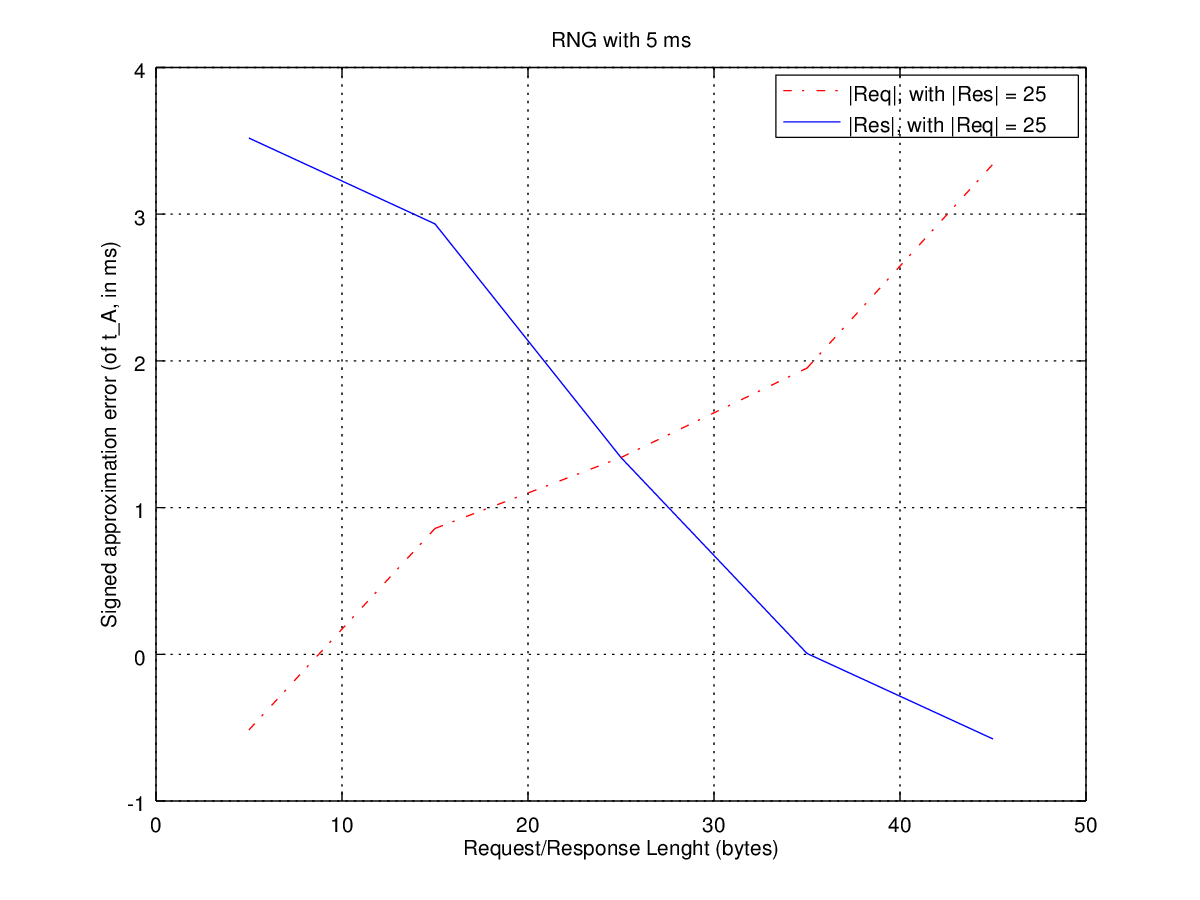
\includegraphics[width=\linewidth]{fig/errwithlen5ms.png}
	\end{subfigure}
	\begin{subfigure}{0.45\linewidth}
		\center
		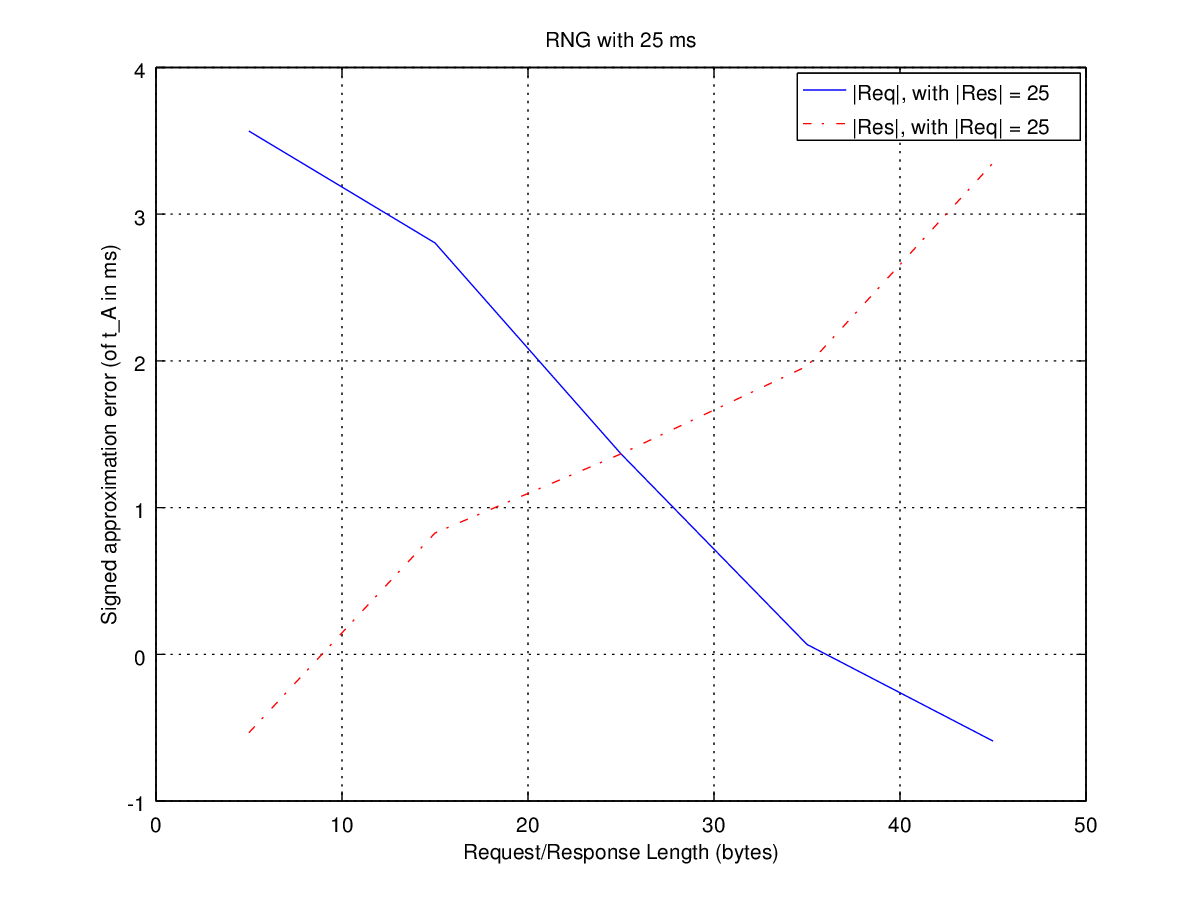
\includegraphics[width=\linewidth]{fig/errwithlen25ms.png}
	\end{subfigure}
	\caption{Affection on $e$ by $|Req|$ and $|Res|$, with Contiki RNG}
	\label{Fig: e by len}
\end{figure}

The result in \Cref{Fig: e by len} suggests that:

\begin{itemize}
	\item $e$ may also multi linearly related to both $|Rea|$ and $|Res|$.
	\item Change of $t_A$ does not seem to affect $e$.
\end{itemize}

Apply multiple linear regression on the results of $t_A = 5$ and $t_A = 25$, we have two regression models:

\begin{equation}
	\hat{e} = 2.007 - 0.111|Req| + 0.088|Res|
\end{equation}

with $R^2 = 0.971$ for $t_A = 5$, and

\begin{equation}
	\hat{e} = 1.962 - 0.111|Req| + 0.089|Res|
\end{equation}

with $R^2 = 0.978$ for $t_A = 25$.

Using the coefficient equality test proposed in \cite{CoeEqTest} on both regression models, the test reports no statistical significance on the coefficients of the regression models. Therefore we re-estimate $e$ using the full data\footnote{Data in both 5 ms group and 25 ms group.} as:

\begin{equation} \label{hate}
	\hat{e} = 1.984 - 0.111|Req| + 0.089|Res|
\end{equation}

with $R^2 = 0.975$.

Recall the fact that the length of packets are constrained by 802.15.4 MTU thus $|Req| \in [0,47]$ and $|Res| \in [0,46]$, we have $\hat{e} \in [-3.233,6.078]$ ms. Although $\hat{e}$ might be hard to predict as it is related to specific application code, in our experiment, $e$ is in a relatively small range. In practice, we would expect that such level of error is tolerable, especially when estimating application code with longer execution time.

\subsection{Differential Analysis}

Sometimes the difference in execution time may also be an interested target to an adversary. 

Denote $\Delta t_A$ to be the difference in application code execution time of two Sessions of the same device, we have:
\begin{equation}\label{Eq: delta t}
	\begin{aligned}
		\Delta t_A &= t_A - t'_A \\
			&= (t_R - t_P) - (t'_R - t'_P) \\
			&= t_R - t'_R - (t_P - t'_P) \\
			&= t_R - t'_R - [(\hat{t}_P - e) - (\hat{t'}_P - e')] \\
			&= t_R - t'_R - \hat{t}_P - \hat{t'}_P - (e - e')
	\end{aligned}
\end{equation}
 
Notice that in \Cref{Eq: delta t}, $t_R$ and $t'_R$ are directly observable from the captured traffic. $\hat{t}_P$ and $\hat{t'}_P$ can solely calculated by $|Req|$ and $|Res|$ which are also directly observable in the packets. This left only $(e-e')$ the uncertainty in \Cref{Eq: delta t}.

On the other hand,  based on the results shown in \Cref{Tbl: Statistical features of eR and eA}, we suppose  the variance of $e$ might be negligible in practice and therefore so is $(e - e')$. In this case, we suggest to approximate \Cref{Eq: delta t} as:
\begin{equation}
	\Delta t \approx t_R - t'_R - \hat{t}_P - \hat{t'}_P = \hat{t}_A - \hat{t'}_A
\end{equation}

However, we consider $(e - e')$ difficult to further quantified, as its value can be affected by the application code (as shown in \Cref{Affection of application code} ) which can hardly be quantified without knowing exactly how it affects the execution time.

\subsection{Execution time of CoAP Implementation}



%DTLS has potentially the best interoperability as it is an variation of the widely used TLS in Internet. However, its design might not fit into the nature of WSN for practical reasons.
%
%\section{Implementation Issues}
%The most practical implementation we found on Contiki OS so far is tinydtls.
%
%tinydtls\cite{tinydtls} currently supports two ciphersuites, namely TLS\_PSK\_WITH\_AES\_128\_CCM\_8 and TLS\_ECDHE\_ECDSA\_WITH\_AES\_128\_CCM\_8. 
%
%However, we encountered several difficulties when trying to set up an encrypted network using tinydtls.
%
%\begin{description}
%\item[Low Computational Power] \hfill \\
%Curve computation requires relatively a large amount of computational power. Even using a relatively powerful platform (CC2538), it still takes minutes to complete a DTLS handshake with
%TLS\_ECDHE\_ECDSA\_WITH\_AES\_128\_CCM\_8.
%
%\item[Low Bandwidth] \hfill \\
%The 6LowPAN standard specifies that the minimum MTU is 127 bytes whilst 67 (87 with LLSEC) bytes are occupied by protocol headers until UDP, which leaves 60 (40 with LLSEC) bytes available for UDP layer payload. This value has been exceeded by several handshake packets even with pre-shared keys. Doing key exchange or even using longer keys only makes this problem worse. Some attempts have been made to solve this issue, e.g. CoDTLS\cite{CoDTLS}\footnote{This draft has been abandoned for some reason we do not know.}. As a result, DTLS is only available on those devices support extra frame length than 6LowPAN requirements.
%
%\item[Code Size] \hfill \\
%The tinydtls fails to fit into some devices, e.g. skymote, as its size of code is too large.
%\end{description}
%
%Therefore although TLS\_PSK\_WITH\_AES\_128\_CCM\_8 is less flexible (and probably less secure) as it uses a pre-shared master secret, it is still considered to be a relatively practical security measure as it requires less resources.
%
%\section{No Multicast Support}
%Some application protocols, such as CoAP, utilises the multicast feature of 6LowPAN whilst TLS is a protocol designated for securing communications between two parties, so is DTLS. To  our knowledge, DTLS does not make any attempt to support multicasting.
%
%\section{Overloading DTLS with LLSEC}
%Adopting both security measures at the same time is possible as they are implemented at different layers. However, it is questionable whether this will bring more security, as both {\it noncoresec} and TLS\_PSK\_WITH\_AES\_128\_CCM\_8 are using 128 bit AES with CCM mode as their cryptographic primitive.
